\section{Letters} 

  \begin{definition}[Typeface, Font]
    A \textbf{typeface} is a design for the 62 alphanumeric characters (26 lowercase + 26 uppercase + 10 digits). A \textbf{font} is a specific variation of that typeface. Some terminology: 
    \begin{enumerate}
      \item The \textbf{baseline} is the line upon which most letters sit. 
      \item The \textbf{mean line}, or the \textbf{x-height}, is the horizontal line 
      \item The \textbf{cap height} is the height of a capital letter above the baseline. 
      \item The \textbf{ascender} is the portion of a lowercase letter that extends above the mean line. 
      \item The \textbf{descender} is the portion of a lowercase letter that extends below the baseline. 
    \end{enumerate}

    \begin{figure}[H]
      \centering 
      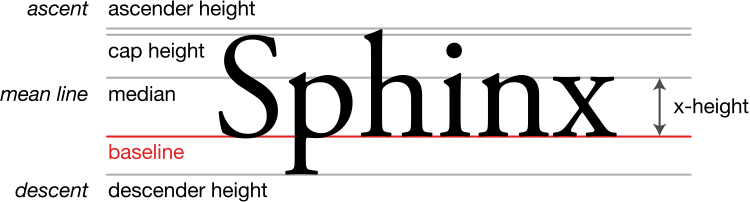
\includegraphics[scale=0.4]{img/typography.png}
      \caption{The anatomy of a font. } 
      \label{fig:typography}
    \end{figure}
  \end{definition}

  Now let's list of a few fonts so that we can refer back to them when talking about properties. 

  \begin{example}[Times]
    Times is a serif typeface commissioned by The Times newspaper of London in 1931 and created by Stanley Morison in collaboration with Victor Lardent. It was designed to be highly legible in small sizes and economical in space usage for newspaper printing. The font became widely popular beyond newspapers and is now one of the most recognizable typefaces in the world. Times New Roman, the most common variant, was adapted by Monotype and later became a default font in many word processors. 
    
    \begin{figure}[H]
      \fontfamily{ptm}\selectfont 
      \huge
      \raggedright
      abcdefghijklmnopqrstuvwxyz \\
      ABCDEFGHIJKLMNOPQRSTUVWXYZ \\
      1234567890
    \end{figure}
  \end{example}

  \begin{example}[Palatino]
    Palatino was designed by Hermann Zapf in 1948 and is named after the 16th-century Italian master of calligraphy Giambattista Palatino. It's a Renaissance old-style serif typeface known for its excellent readability and elegant appearance. Palatino is wider than many serif fonts, making it particularly suitable for body text in books and academic documents. 
    
    \begin{figure}[H]
      \fontfamily{ppl}\selectfont
      \huge
      \raggedright
      abcdefghijklmnopqrstuvwxyz \\
      ABCDEFGHIJKLMNOPQRSTUVWXYZ \\
      1234567890
    \end{figure}
  \end{example}

  \begin{example}[Computer Modern Roman]
    Computer Modern Roman is the default serif font in LaTeX, designed by Donald Knuth specifically for the TeX typesetting system in the 1980s. Based on Monotype Modern 8A, it was created to provide optimal readability for mathematical and scientific documents. 
    
    \begin{figure}[H]
      \huge
      \raggedright
      abcdefghijklmnopqrstuvwxyz \\
      ABCDEFGHIJKLMNOPQRSTUVWXYZ \\
      1234567890
    \end{figure}
  \end{example}

  \begin{example}[Helvetica]
    Helvetica was created by Swiss typeface designer Max Miedinger in 1957. It's a neo-grotesque sans-serif typeface that became one of the most widely used fonts in the world, known for its clean, modern appearance and neutral character. Originally called Neue Haas Grotesk, it was renamed Helvetica (meaning "Swiss" in Latin) for international marketing. 
    
    \begin{figure}[H]
      \fontfamily{phv}\selectfont 
      \huge
      \raggedright
      abcdefghijklmnopqrstuvwxyz \\
      ABCDEFGHIJKLMNOPQRSTUVWXYZ \\
      1234567890
    \end{figure}
  \end{example}

  \begin{example}[Courier]
    Courier was designed by Howard "Bud" Kettler in 1955 for IBM typewriters. It's a monospaced slab serif typeface where every character occupies the same horizontal space, originally created to mimic typewriter output. Courier became the standard font for screenplays and is widely used in programming and technical documentation. 
    
    \begin{figure}[H]
      \fontfamily{pcr}\selectfont
      \huge
      \raggedright
      abcdefghijklmnopqrstuvwxyz \\
      ABCDEFGHIJKLMNOPQRSTUVWXYZ \\
      1234567890
    \end{figure}
  \end{example}

  \begin{example}[Bookman]
    Bookman Old Style was originally designed by Alexander Phemister in 1860 and later refined by various foundries. It's a serif typeface with strong, sturdy letterforms and generous spacing, making it highly legible even at small sizes. The font has a somewhat informal, friendly character while maintaining professional appearance. It's particularly popular in book publishing. 
    
    \begin{figure}[H]
      \fontfamily{pbk}\selectfont
      \huge
      \raggedright
      abcdefghijklmnopqrstuvwxyz \\
      ABCDEFGHIJKLMNOPQRSTUVWXYZ \\
      1234567890
    \end{figure}
  \end{example}

  \begin{example}[Charter]
    Charter was designed by Matthew Carter in 1987 specifically for low-resolution printing and fax transmission. Despite being created for technical constraints, it became appreciated for its excellent readability and robust character shapes. Charter is particularly effective in challenging printing conditions and remains highly legible across various media. 
    
    \begin{figure}[H]
      \fontfamily{bch}\selectfont
      \huge
      \raggedright
      abcdefghijklmnopqrstuvwxyz \\
      ABCDEFGHIJKLMNOPQRSTUVWXYZ \\
      1234567890
    \end{figure}
  \end{example}
  
  Now let's talk about some properties. 

\subsection{Size} 

  \begin{definition}[Size]
    The \textbf{size} of a font is the \textit{height} of its characters. 
  \end{definition} 

  \begin{theorem}[Height]
    For a given height, a circle and a triangle appear smaller than a square. For them to be the same height, they must extend slightly beyond the cap height and baseline. 

    \begin{figure}[H]
      \centering 
      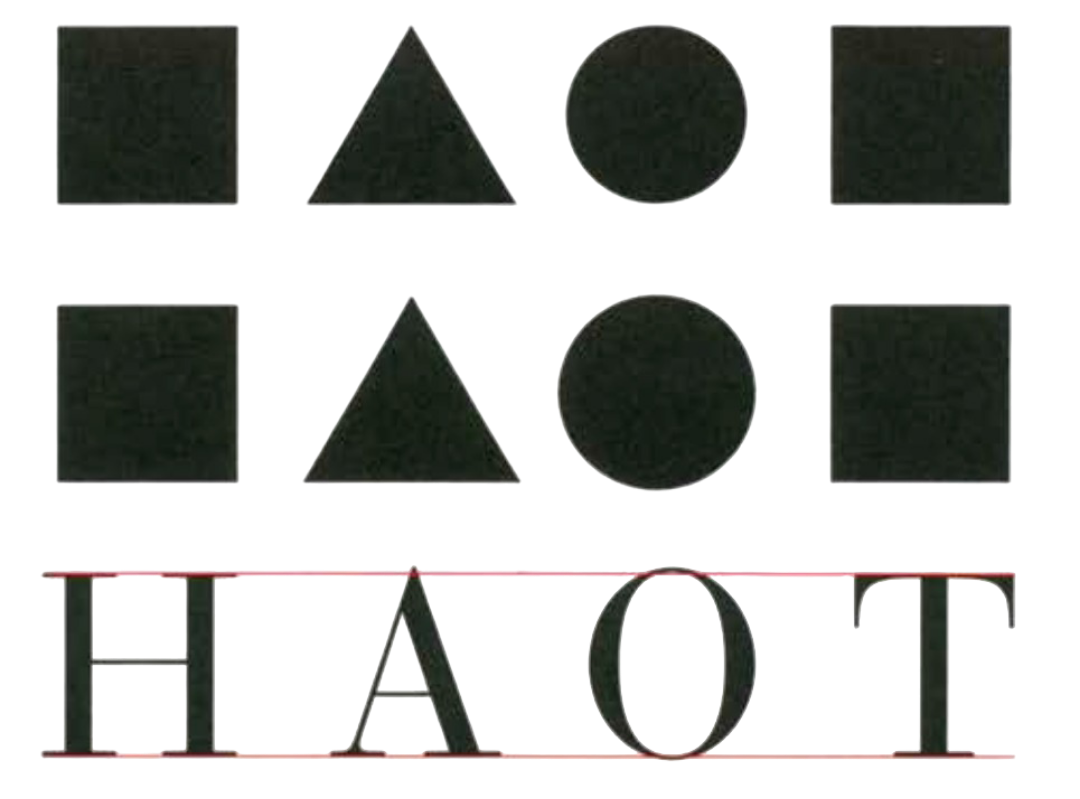
\includegraphics[scale=0.3]{img/size.png}
      \caption{} 
      \label{fig:size}
    \end{figure}
  \end{theorem} 

  \begin{theorem}[Width]
    Small sizes of type need to be proportionally wider than larger sizes. This is an optical requirement that is essential for readability.\footnote{Even in our own handwriting: the larger the writing, the narrower the individual letters. } 
  \end{theorem}

  \begin{theorem}[Height of Lowercase vs Uppercase]
    The size of capital letters can be quite overwhelming, and so the size of capital letters should be somewhat lower than the lowercase ascenders. 

    \begin{figure}[H]
      \centering 
      
\includegraphics[scale=0.4]{img/ascender.png}
      \caption{The capitals of many typefaces are lower than the lowercase ascenders.} 
      \label{fig:ascender}
    \end{figure}
  \end{theorem}

  These ascenders are quite important. 

  \begin{theorem}
    Recognizing a letter from the upper half is much easier than the lower half.
    \begin{figure}[H]
      \centering 
      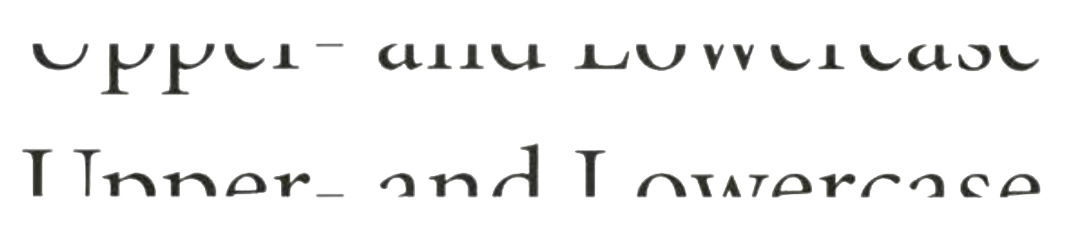
\includegraphics[scale=0.4]{img/half_erased}
      \caption{} 
      \label{fig:half_erased}
    \end{figure}
  \end{theorem}

  \begin{figure}[H]
    \centering 
    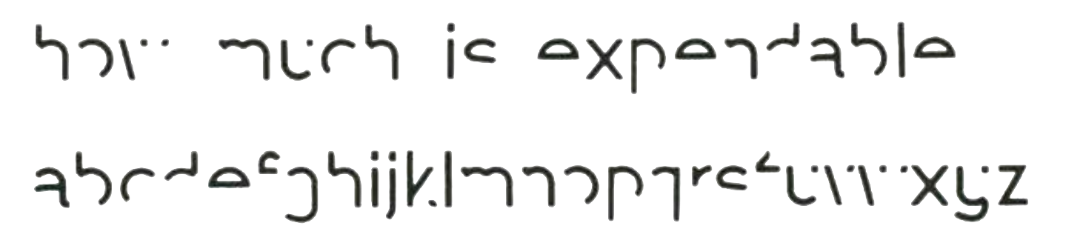
\includegraphics[scale=0.4]{img/some_erased.png}
    \caption{A partial result of an experiment with which Brian Coe attempted to discover how much of a lowercase letter can be deleted before it becomes unreadable.} 
    \label{fig:some_erased}
  \end{figure}

\subsection{Weight}

  Bold 

  \begin{theorem}[Weight]
    For a given weight of line, a horizontal line appears heavier than a vertical line. To achieve optically balanced verticals and horizontals, which appear to be of the same weight, the horizontal must be somewhat narrower.  

    \begin{figure}[H]
      \centering
      \begin{subfigure}[b]{0.48\textwidth}
        \centering
        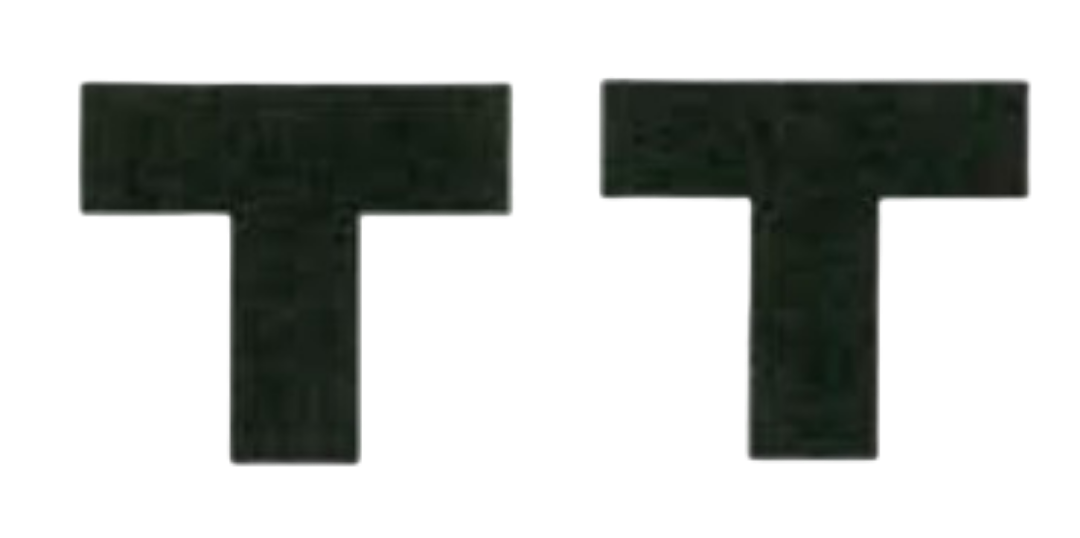
\includegraphics[width=\textwidth]{img/t.png}
        \caption{Uncorrected vs corrected T.}
        \label{fig:t}
      \end{subfigure}
      \hfill 
      \begin{subfigure}[b]{0.48\textwidth}
        \centering
        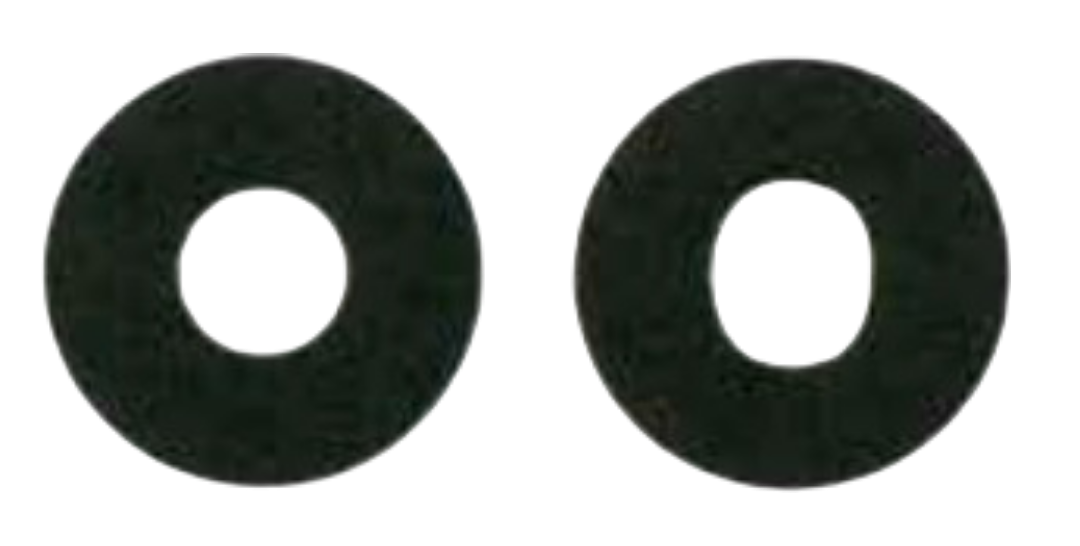
\includegraphics[width=\textwidth]{img/o.png}
        \caption{Uncorrected vs corrected O.}
        \label{fig:o}
      \end{subfigure}
      \caption{}
      \label{fig:weight}
    \end{figure}
  \end{theorem} 

\subsection{Slant}

  Italicizing. 

\subsection{Symmetry and Radiation} 

  \begin{theorem}[Symmetry]
    The mathematically equal horizontal division of an area produces an upper half that appears larger than the lower half. To produce two halves of a naturally equal size, the dividing line must lie above the mathematical center, at what is known as the \textbf{optical center}.  

    \begin{figure}[H]
      \centering
      \begin{subfigure}[b]{0.43\textwidth}
        \centering
        
\includegraphics[width=0.86\textwidth]{img/e.png}
        \caption{The middle horizontal bar is mathematically centered on the left and optically on the right. }
        \label{fig:e}
      \end{subfigure}
      \hfill 
      \begin{subfigure}[b]{0.48\textwidth}
        \centering
        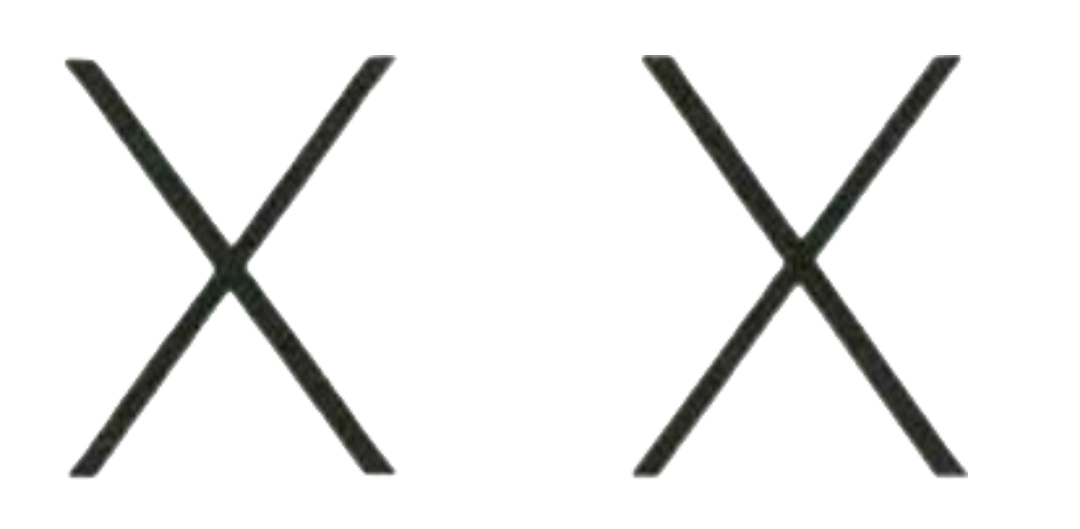
\includegraphics[width=\textwidth]{img/x.png}
        \caption{The intersection is mathematically centered on the left and optically centered on the right. }
        \label{fig:x}
      \end{subfigure}
      \caption{}
      \label{fig:symmetry}
    \end{figure}
  \end{theorem} 

\subsection{Radiation}

  \begin{theorem}[Radiation]
    Where curves intersect with straight lines or with other curves, or where two diagonals meet, lumps will occur, which, unless corrected, will disfigure the letter and make the composition appear blobby. 

    \begin{figure}[H]
      \centering
      \begin{subfigure}[b]{0.45\textwidth}
        \centering
        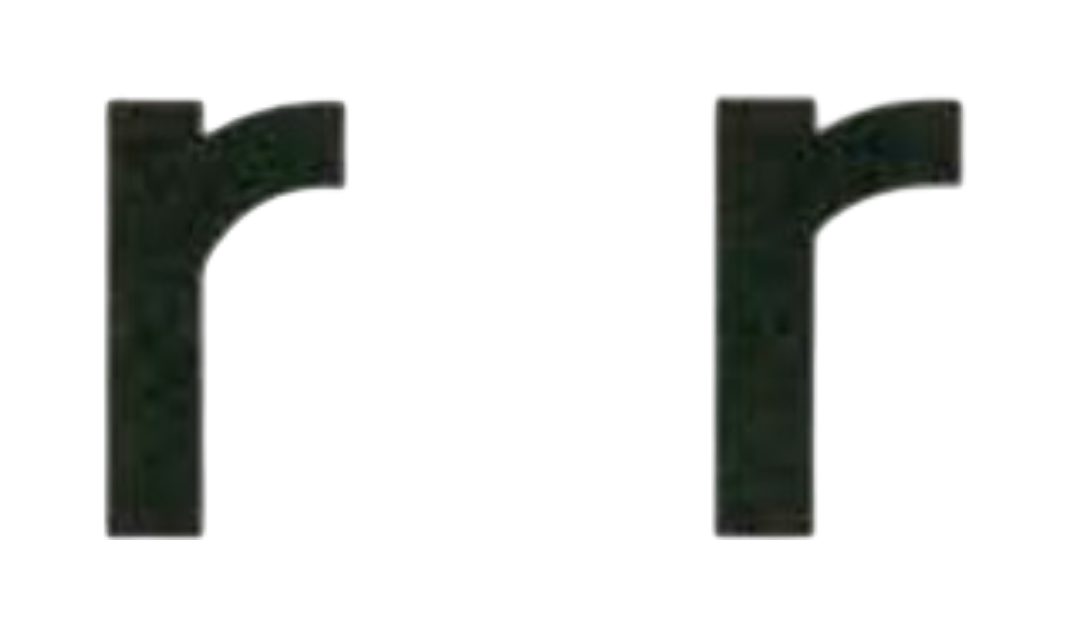
\includegraphics[width=\textwidth]{img/r.png}
        \caption{}
        \label{fig:r}
      \end{subfigure}
      \hfill 
      \begin{subfigure}[b]{0.48\textwidth}
        \centering
        
\includegraphics[width=\textwidth]{img/v.png}
        \caption{}
        \label{fig:v}
      \end{subfigure}
      \caption{}
      \label{fig:blob}
    \end{figure}
  \end{theorem}

\subsection{Serifs} 

  Serifs and sans serifs


